\documentclass{oci}
\usepackage[utf8]{inputenc}
\usepackage{lipsum}

\title{Suma de ejemplo}

\begin{document}
\begin{problemDescription}
  Finalmente ha llegado el día que todos estaban esperando: la fase final de la Olimpiada de
  Cachipun Internacional (OCI). En esta competencia, $n$ oponentes se enfrentan en $k$ rondas de combate
  todos-contra-todos, donde en cada ronda, cada participante elige una opción entre piedra, 
  papel y tijera. Cada jugador gana $1$ punto por cada contrincante que venció, pierde $1$ por cada 
  contrincante que lo venció, y los empates no afectan su puntuación.

  Por ejemplo, en una ronda con $5$ jugadores, donde tú eres el jugador 1 y los jugadores juegan de 
  la siguiente forma:

  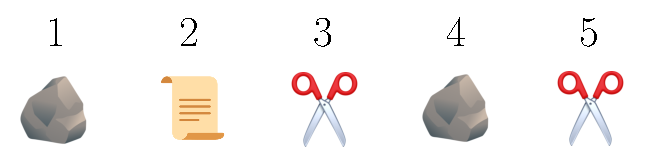
\includegraphics{ronda.eps}

  Tú le ganarías a los jugadores 3 y 5, obteniendo $2$ puntos, pierdes contra el jugador 2 que resta $1$ 
  punto, y empatas con el jugador 4, para un resultado total de $1$ punto a tu favor.

  Normalmente, el registro de los puntos se maneja utilizando el Cachipun Management System (CMS), 
  sin embargo, Diego encontró una vulnerabilidad en el software, y como no hay tiempo suficiente 
  para arreglarlo, la administración decidió pedirte a ti que crees un programa que lo sustituya.

  Quedan menos de 4 horas para que comience la competencia, ¿podrás salvar la OCI?
\end{problemDescription}

\begin{inputDescription}
  Te dan $n (2 \leq n \leq 1000), k (1 \leq k \leq 1000)$ y la matriz de $k \times n$, 
  donde la $i$-ésima fila representa la $i$-ésima ronda, y la $j$-ésima columna representa la jugada del $j$-ésimo jugador.
  El carácter R representa roca, P representa papel y T tijeras.
\end{inputDescription}

\begin{outputDescription}
  Debes imprimir $n$ números, donde el $i$-ésimo número corresponde a la puntuación final del jugador $i$.
\end{outputDescription}

\begin{scoreDescription}
  \subtask{20} Se probarán varios casos de prueba donde $n = 2$, es decir, hay exactamente $2$ jugadores.
  \subtask{40} Se probarán varios casos de prueba donde $n \leq 100$.
  \subtask{40} Se probarán varios casos de prueba sin restricciones adicionales.
\end{scoreDescription}

\begin{sampleDescription}
\sampleIO{sample-1}
\sampleIO{sample-2}
\end{sampleDescription}

\end{document}
